\begin{Exercise}[title=(*) Étude d'un cyclotron]
  \begin{minipage}{.6\linewidth}
    Un cyclotron est une instrument qui sert à accélérer des particules chargées, permettant ensuite de réaliser des expériences de physique nucléaire. Dans ce problème les particules chargée sont des protons de masse \gdr{m_p}{1.67e-27}{\kg} et de charge électrique \gdr{q_p}{1,6e-19}{C}.
    Le cyclotron est formé de deux demis-cylindres conducteurs creux appelé "dees" et séparée par un intervalle étroit. Un champ magnétique uniforme $B$ règne à l'intérieur de chaque "dee" sa direction est parallèle à l'axe de ces demis cylindre et \gdr{B}{1,0}{T}.

    un champ électrique $\vec{E}$ variable dans le temps, peut être établi dans l'intervalle étroit qui sépare les "dees". Il permet d'accélérer les protons chaque fois qu'il pénètre dans cet intervalle. Ce champ électrique variable est obtenu e, appliquant une tension créneau oscillant entre $-U_M$ et $U_M$ et de fréquence $f$ entre deux dees: \gdr{U_M}{2.e3}{V}.

	On donne le schéma simplifié d'un cyclotron sur la figure ci-contre.
  \end{minipage}\hspace{.05\linewidth}
  \begin{minipage}{.3\linewidth}
    \includegraphics[width=\textwidth]{cyclotron.png}
  \end{minipage}
  \Question Le proton entre dans le dee 1 avec une vitesse initiale d'injection $\vec{v_0}$ perpendiculaire à l'axe des demi-cylindres.
		\subQuestion Faire un bilan des forces et les représenter sur un schéma.
		\subQuestion En admettant que le mouvement est plan, montrer que la norme de la vitesse est constante.
		\subQuestion En admettant que le mouvement est circulaire, déterminer son rayon.
		\subQuestion Exprimer la longueur et calculer le temps nécessaire au proton pour effectuer un demi-tours du cyclotron. Commentaire.
		\Question Le proton après un demi tour dans le dee , entre dans l'intervalle étroit où il est accéléré par le champs électrique considérer comme constant, maximum et colinéaire au vecteur vitesse du proton durant son passage.
		\subQuestion Exprimer littéralement puis calculer la variation  d'énergie cinétique du proton à chaque passage dans l'intervalle.
		\subQuestion Préciser  si le rayon  de la trajectoire augmente ou diminue à chaque fois qu'il traverse l'intervalle .
		\Question La vitesse d'injection du proton étant considérée pratiquement nulle , on désire que sa vitesse 	atteigne \gdr{}{2e4}{\km\per\s}
		\subQuestion Calculer le nombre de tour nécessaire pour atteindre cette vitesse.
		\subQuestion Calculer la valeur du rayon à partir duquel les protons ayant acquis la vitesse désirée son extrait, en considérant qu'il sont injectée à proximité du centre du cycloctron.
\end{Exercise}
\begin{Answer}
		\Question
		\subQuestion $f= q_p\vec{V_0}\wedge\vec{B}$
		\subQuestion $\dd{E_c}{t} = (q\vec{v},\vec{B},\vec{v})=0$
		\subQuestion PFD dans un MCU : $m\frac{v^2}{R_0} = q_Pv_0B$ puis $R_0=\frac{m_pv_0}{q_pB}$
		\subQuestion ce temps est indépendant de la vitesse d'entree dans le dee. \gdr{\Delta}{3,28e-8}{s}.
		\Question
		\subQuestion on veux $f= \frac{1}{2\Delta t} =$\gdr{\frac{q_PB}{2\pi m_p}}{15.2}{MHz}.
		\subQuestion \gdr{\Delta E_c}{3,2e-16}{J}\gdr{}{2e3}{eV} à chaque passage dans l'entrefer.
		\Question
		\subQuestion il faut $N=\frac{E_c}{\Delta E_c}$ passage dans l'entrefer soit $n \simeq 500 tr$
		\subQuestion \gdr{R = \frac{m_pv_f}{q_pB}}{0,209}{m} passage à une distance $D=2R$ du centre, à 41,8cm
\end{Answer}
